\begin{frame}{Extension: Proactive Secret Sharing \cite{herzberg1995proactive}}
	\begin{itemize}
		\item Motivation: long-lived secrets face \textbf{perpetual leakage} (devices get compromised over time).
		\item Proactive SSS periodically \textbf{refreshes shares} without changing the underlying secret \(s\).
		\item Security intuition: as long as the adversary does not control too many parties \emph{within one refresh period}, the secret remains protected.
	\end{itemize}

	\begin{figure}
		\centering
		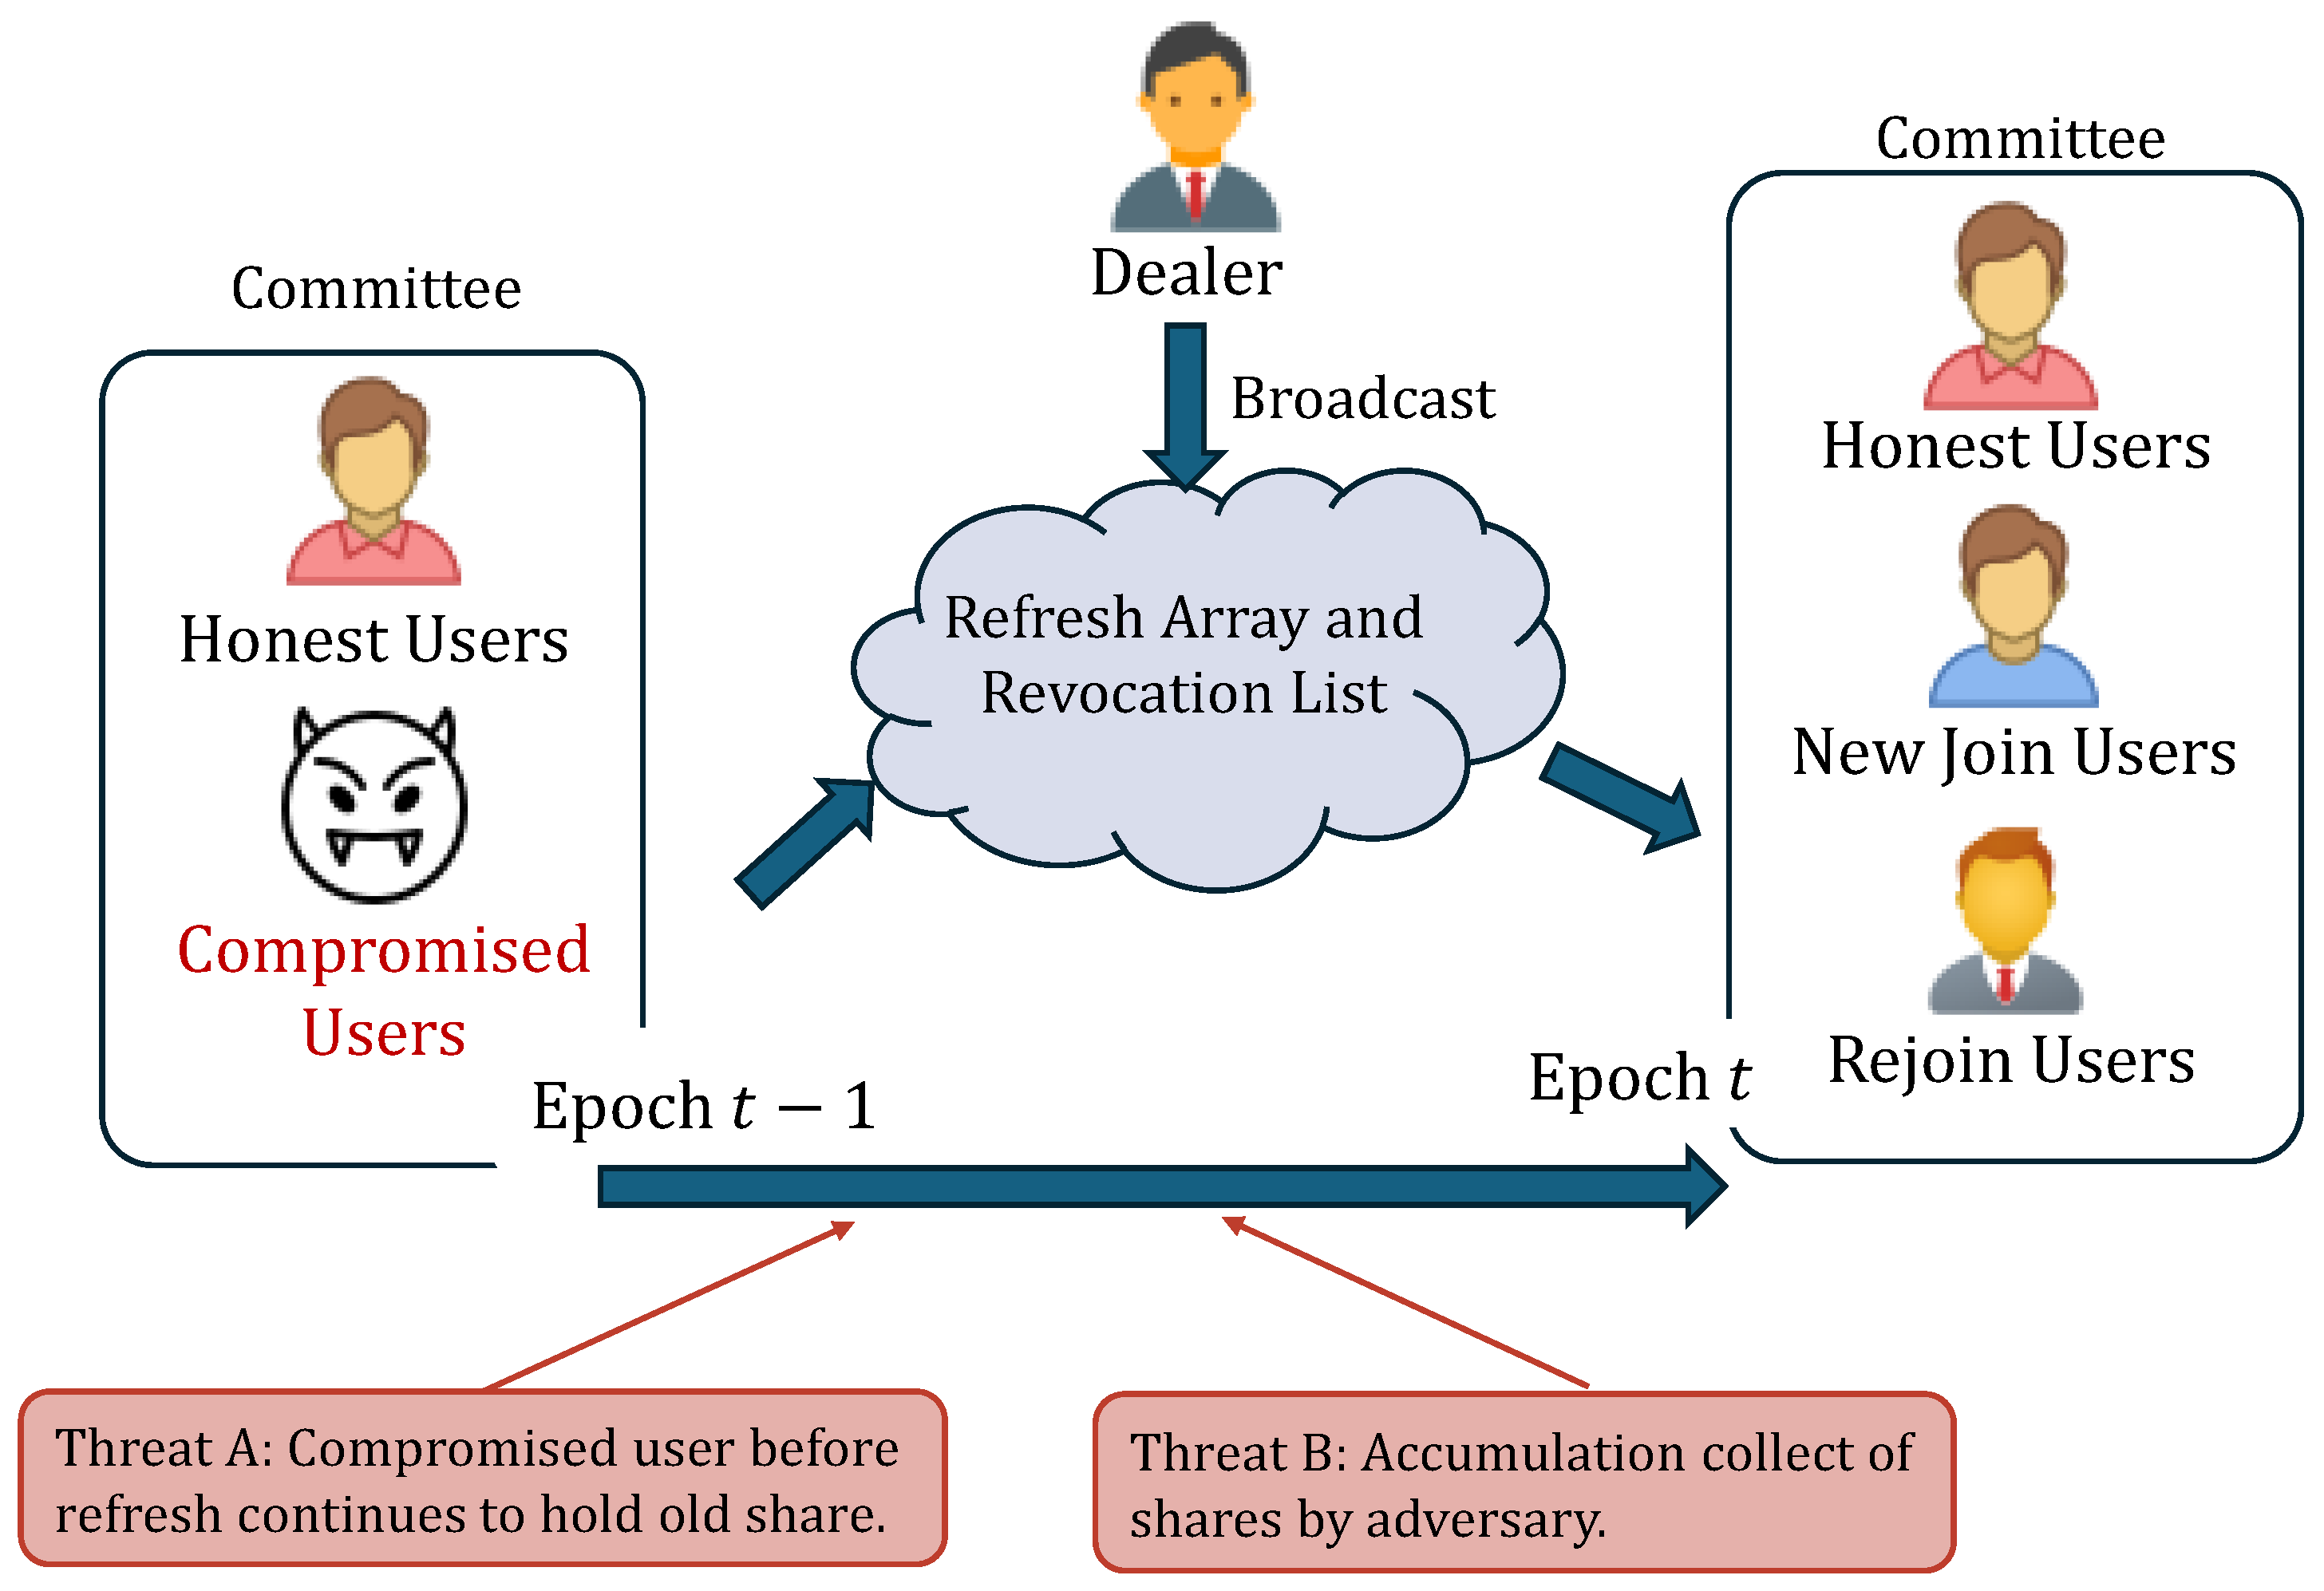
\includegraphics[scale=0.5]{fig/fig-role-based-proactive-secret-sharing.png}
		\caption{Proactive Secret Sharing - Refresh over Time}
	\end{figure}
\end{frame}

\begin{frame}{Extension: Quantum Secret Sharing (High-level) \cite{gottesman2000theory}}
	\begin{itemize}
		\item Quantum secret sharing distributes a quantum state so only authorized sets can reconstruct it.
		\item Connects to quantum error-correcting codes: authorized sets can recover; unauthorized sets learn nothing.
		\item Relevance: shows the access-structure viewpoint generalizes beyond classical secrets.
	\end{itemize}
\end{frame}
